% ****** Start of file apssamp.tex ******
%
%   This file is part of the APS files in the REVTeX 4.1 distribution.
%   Version 4.1r of REVTeX, August 2010
%
%   Copyright (c) 2009, 2010 The American Physical Society.
%
%   See the REVTeX 4 README file for restrictions and more information.
%
% TeX'ing this file requires that you have AMS-LaTeX 2.0 installed
% as well as the rest of the prerequisites for REVTeX 4.1
%
% See the REVTeX 4 README file
% It also requires running BibTeX. The commands are as follows:
%
%  1)  latex apssamp.tex
%  2)  bibtex apssamp
%  3)  latex apssamp.tex
%  4)  latex apssamp.tex
%
\documentclass[%
 reprint,
%superscriptaddress,
%groupedaddress,
%unsortedaddress,
%runinaddress,
%frontmatterverbose, 
%preprint,
%showpacs,preprintnumbers,
%nofootinbib,
%nobibnotes,
%bibnotes,
 amsmath,amssymb,
 aps,
%pra,
%prb,
%rmp,
%prstab,
%prstper,
%floatfix,
10.5pt,
]{revtex4-1}

\usepackage{graphicx}% Include figure files
\usepackage{subfigure}
\usepackage{multirow}
\usepackage{array}
\usepackage{dcolumn}% Align table columns on decimal point
\usepackage{bm}% bold math
%\usepackage{hyperref}% add hypertext capabilities
%\usepackage[mathlines]{lineno}% Enable numbering of text and display math
%\linenumbers\relax % Commence numbering lines

%\usepackage[showframe,%Uncomment any one of the following lines to test 
%%scale=0.7, marginratio={1:1, 2:3}, ignoreall,% default settings
%%text={7in,10in},centering,
%%margin=1.5in,
%%total={6.5in,8.75in}, top=1.2in, left=0.9in, includefoot,
%%height=10in,a5paper,hmargin={3cm,0.8in},
%]{geometry}

\usepackage{xeCJK}
%\setCJKmainfont[ItalicFont={KaiTi}, BoldFont={KaiTi}]{KaiTi}
\usepackage{textcomp}
\usepackage{chemfig}
\usepackage[version=4]{mhchem}
\usepackage{fontspec}
\usepackage{listings}
\usepackage{xcolor}
\usepackage{xcolor} % 定制颜色
\definecolor{mygreen}{rgb}{0,0.6,0}
\definecolor{mygray}{rgb}{0.5,0.5,0.5}
\definecolor{mymauve}{rgb}{0.58,0,0.82}
\lstset{
backgroundcolor=\color{white},      % choose the background color
basicstyle=\footnotesize\ttfamily,  % size of fonts used for the code
columns=fullflexible,
tabsize=4,
breaklines=true,               % automatic line breaking only at whitespace
captionpos=b,                  % sets the caption-position to bottom
commentstyle=\color{mygreen},  % comment style
escapeinside={\%*}{*)},        % if you want to add LaTeX within your code
keywordstyle=\color{blue},     % keyword style
stringstyle=\color{mymauve}\ttfamily,  % string literal style
frame=single,
rulesepcolor=\color{red!20!green!20!blue!20},
% identifierstyle=\color{red},
language=Mathematica,
}

\usepackage[normalem]{ulem}

\newcommand{\chuhao}{\fontsize{42pt}{44.9pt}\selectfont}    % 初号, 1.5倍行距
\newcommand{\xiaochu}{\fontsize{30pt}{40pt}\selectfont}    % 小初, 1.5倍行距
\newcommand{\yihao}{\fontsize{26pt}{36pt}\selectfont}    % 一号, 1.4倍行距
\newcommand{\erhao}{\fontsize{22pt}{28pt}\selectfont}    % 二号, 1.25倍行距
\newcommand{\xiaoer}{\fontsize{18pt}{18pt}\selectfont}    % 小二, 单倍行距
\newcommand{\sanhao}{\fontsize{16pt}{24pt}\selectfont}    % 三号, 1.5倍行距
\newcommand{\xiaosan}{\fontsize{15pt}{22pt}\selectfont}    % 小三, 1.5倍行距
\newcommand{\sihao}{\fontsize{14pt}{21pt}\selectfont}    % 四号, 1.5倍行距
\newcommand{\sihaox}{\fontsize{14pt}{28pt}\selectfont}    % 四号, 1.5倍行距
\newcommand{\banxiaosi}{\fontsize{13pt}{19.5pt}\selectfont}    % 半小四, 1.5倍行距
\newcommand{\xiaosix}{\fontsize{12pt}{24pt}\selectfont} 	% 小四, 1.5倍行距
\newcommand{\xiaosi}{\fontsize{12pt}{18pt}\selectfont}     
\newcommand{\dawuhao}{\fontsize{11pt}{11pt}\selectfont}    % 大五号, 单倍行距
\newcommand{\wuhao}{\fontsize{10.5pt}{10.5pt}\selectfont}    % 五号, 单倍行距
\newcommand{\xiaowu}{\fontsize{9pt}{9pt}\selectfont}    % 五号, 单倍行距

%\usepackage[fntef]{ctexcap}
%\CTEXsetup[number={\chinese{section}、},format={\Large\bfseries}]{section}
%\setCJKfamilyfont{fangsong}{FangSong}                      %仿宋2312 fs  
%\newcommand{\fangsong}{\CJKfamily{fangsong}}  

\usepackage{wrapfig}
\usepackage{fancyhdr}
\usepackage{fancybox}   


\usepackage{tikz}
\usepackage{circuitikz}



\newcommand{\bra}[1]{\langle #1 |}
\newcommand{\ket}[1]{| #1 \rangle}
\newcommand{\bracket}[2]{\langle #1 | #2 \rangle}
\newcommand{\bracketl}[3]{\langle #1 | #2 | #3 \rangle}
\newcommand{\func}{\mathrm \,}
\newcommand{\define}[2]{
	\begin{definition}
	\begin{description}
	\item[#1]
	#2
	\end{description}
	\end{definition}
}

\newcommand{\sch}{Schr\"odinger}
\newcommand{\grad}{\nabla}
\newcommand{\ueq}{\neq}
\newcommand{\celsius}{\ensuremath{^\circ\hspace{-0.09em}\mathrm{C}}}
\newcommand{\unit}[2]{$#1 \, \mathrm{#2}$}

\begin{document}

%\preprint{APS/123-QED}

\title{Measurement of surface tension and isothermal adsorption}% Force line breaks with \\
%\thanks{A footnote to the article title}% give thanks

\author{Rui Li}
 %\altaffiliation[Also at ]{Physics Department, XYZ University.}%Lines break automatically or can be forced with \\
%\author{Second Author}%
%\email{3160102098@zju.edu.cn}
\affiliation{%
 Qiushi science class (chemistry)\\
 Chu Kochen Honor College
}%

%\collaboration{MUSO Collaboration}%\noaffiliation

%\author{Zong Wei Huang}
% \homepage{http://www.Second.institution.edu/~Charlie.Author}
%\affiliation{
% Second institution and/or address\\
% This line break forced% with \\
%}%
%\affiliation{
%Qiushi science class (chemistry)\\
% Chu Kochen Honor College
%}%
%\author{Delta Author}
%\affiliation{%
% Authors' institution and/or address\\
% This line break forced with \textbackslash\textbackslash
%}%

%\collaboration{CLEO Collaboration}%\noaffiliation

%\date{\today}% It is always \today, today,
             %  but any date may be explicitly specified

\begin{abstract}
Surface tension of the different concentration of n-butanol solutions are obtained \emph{via} forming bubbles and measuring the deviation of pressure. The saturated adsorption amount as well as the cross-sectional area of n-butanol is also obtained in the experiment.
\begin{description}
\item[Keywords]
surface tension, n-butanol, adsorption
\end{description}
\end{abstract}

%\pacs{Valid PACS appear here}% PACS, the Physics and Astronomy
                             % Classification Scheme.
%\keywords{Suggested keywords}%Use showkeys class option if keyword
                              %display desired
\maketitle

\tableofcontents

\section{Introduction}
Surface tension is the elastic tendency of a fluid surface which makes it acquire the least surface area possible, which arises from the pulling interaction between molecules in the fluid. The tendency of least surface area leads to an extra pressure towards the center, which can be given by
\begin{equation}
\Delta p = \gamma (\frac{1}{R_x}+\frac{1}{R_y})
\end{equation}
known as the Young-Laplace equation, where $\gamma$ represents the surface tension, and $R_x,\,R_y$ the radii of curvature in two arbitrary orthogonal axes that are parallel to the surface. Or simply,
\begin{equation}
\Delta p = \frac{2 \gamma}{R}
\end{equation}
for a spherical surface. 

When the mouth of a capillary touches the surface of a fluid and there exists a deviation of pressure between the inner and the outer side of capillary, a bubble can be formed on the mouth of the capillary, exerting an extra pressure towards the center of the bubble, which can be detected by measuring the pressure outside the capillary. The maximum radius of the bubble is dominated by the inner radius of the capillary, thus it remains constant for different types of fluids.

The Gibbs adsorption isotherm for multicomponent systems is an equation used to relate the changes in concentration of a component in contact with a surface with changes in the surface tension, which results in a corresponding change in surface energy. For a binary system, the Gibbs adsorption equation in terms of surface excess is 
\begin{equation}
- \mathrm { d } \gamma = \Gamma _ { 1 } \mathrm { d } \mu _ { 1 } + \Gamma _ { 2 } \mathrm { d } \mu _ { 2 }
\end{equation}
If the solute is relatively low in content, it can be approximated that $d\mu =0$ for the solvent and 
\begin{equation}
d \mu = RT \,d\ln c
\end{equation}
for the solute. Then
\begin{equation}
\Gamma = - \frac{c}{RT} \left(\frac{\partial \gamma}{\partial c}\right)_T
\end{equation}

From another perspective, the surface adsorption can be regarded as a equilibrium
\begin{center}
\ce{A(g) + S <-> AS}
\end{center}
which represents the process of adduction between the two substances, \ce{A(g)}~being the gas molecule in the gas phase, while \ce{AS}~is the adduction product of the gas molecule and the molecule on the surface of the condensed substance.

\begin{figure}
\centering
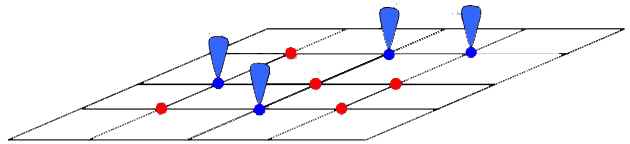
\includegraphics[width=0.45\textwidth]{figures/Langmuir_Adsorption_Model.jpg}
\caption{A simple graphic representation of the Langmuir adsorption model, where the red dots signify the unoccupied area, the blue points the occupied area.}
\end{figure}

Langmuir\cite{langmuir1918adsorption} supposed that the adsorption rate is proportionl to the pressure of gas A and the area on the surface which haven't been occupied, while the desorption rate is proportional to the area occupied, which is shown by
\begin{equation}
k_{ad} p S_0 = k_{de} S_1
\end{equation}
where $k_{ad},k_{de}$ represent the reaction rate constant of the adsorption and the desorption respectively, $S_0,S_1$ the unoccupied and the occupied area, and $p$ the pressure of gas A in bulk phase.

Define the occupied percentage $\theta$
\begin{equation}
\theta = \frac{S_1}{[S]} = \frac{S_1}{S_0+S_1} = \frac{k_{ad}p}{k_{ad}p+k_{de}}
\end{equation}
and the adsorption equilibrium constant $K=\frac{k_{ad}}{k_{de}}$, then
\begin{equation}
\theta = \frac{Kp}{1+Kp}
\end{equation}
and considering that $p \propto c$ for a dilute solution, then it can be deduced that
\begin{equation}
\Gamma = \Gamma_\infty \frac{Kc}{1+Kc}
\end{equation}
or
\begin{equation}
\frac{c}{\Gamma} = \frac{c}{\Gamma_\infty} + \frac{1}{K \Gamma_\infty}
\end{equation}


\section{Methods and Procedures}
A series of different concentration of n-butanol water solutions are prepared. The surface tension measurement apparatus, consisting of a dropping funnel, a digital pressure measurement device, a capillary and a cealed container, is put into a thermostat with temperature constant at 25 \celsius, and dropped into the different concentration of n-butanol solutions, with the surface of which touches the capillary precisely. Water in teh dropping funnel is dropped at a constant rate, so that the bubbles can form at a tempered rate, and the maximum drop of pressure is measured and recorded.

\section{Results and Analysis}
\begin{table}
\centering
\caption{The maximum deviation of pressure for different concentration of n-butanol solutions at 25 \celsius}
\begin{tabular}{cc|cc|cc}\hline
$c$/M & $\Delta p$/Pa & $c$/M & $\Delta p$/Pa & $c$/M & $\Delta p$/Pa \\ \hline
 0.00 & 72.1 & 0.01 & 68.1 & 0.02 & 63.7 \\
 0.04 & 60.4 & 0.06 & 56.8 & 0.09 & 53.6 \\
 0.12 & 50.6 & 0.16 & 46.9 & 0.20 & 44.5 \\\hline
\end{tabular}
\label{data}
\end{table}

\begin{figure}
\centering
\subfigure[A]{
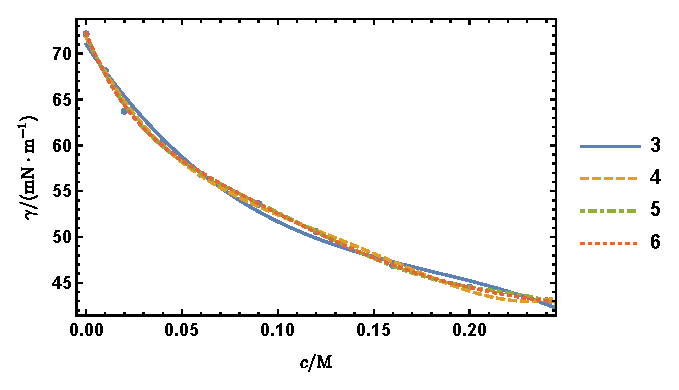
\includegraphics[width=0.45\textwidth]{figures/powerfit.eps}
}
\subfigure[B]{
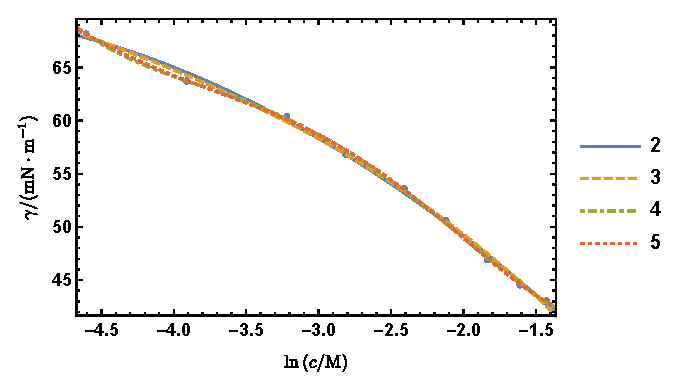
\includegraphics[width=0.45\textwidth]{figures/Logfit.eps}
}
\subfigure[C]{
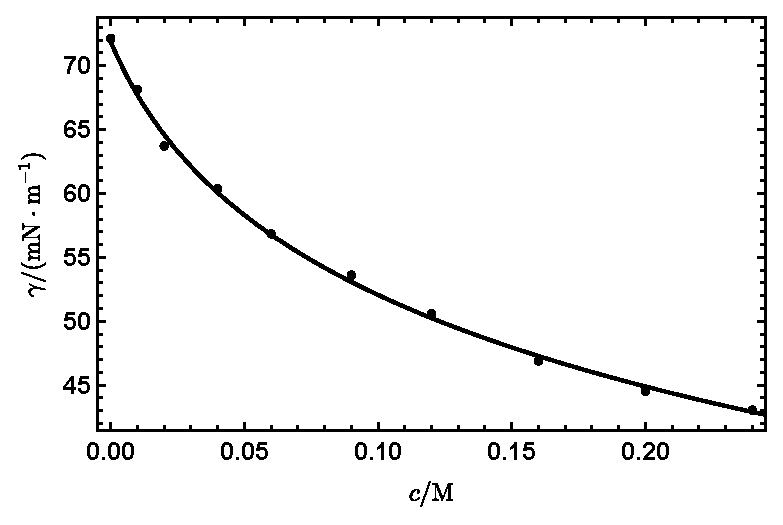
\includegraphics[width=0.45\textwidth]{figures/specialfit.eps}
}
\caption{The fitting of the experimental data using different methods, where\\A: power series\\B: logarithm series\\C: $C_1+C_2\ln{(c + C_3)}$\\with legends representing the degrees of the series applied in the fitting.}
\label{fit}
\end{figure}

\begin{figure}
\centering
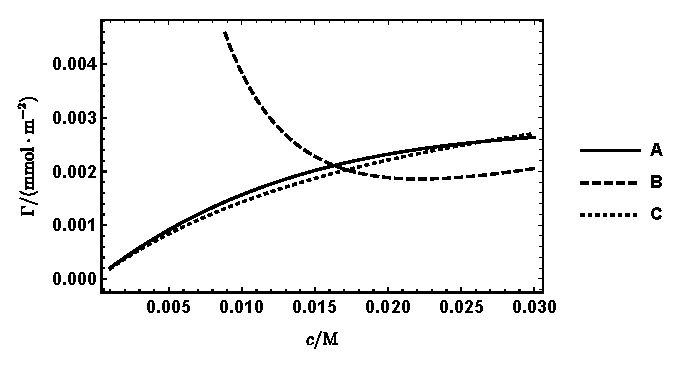
\includegraphics[width=0.45\textwidth]{figures/Gibbs.eps}
\caption{$\Gamma-c$ plots for three different fitting methods}
\label{Gibbs}
\end{figure}

\begin{figure}
\centering
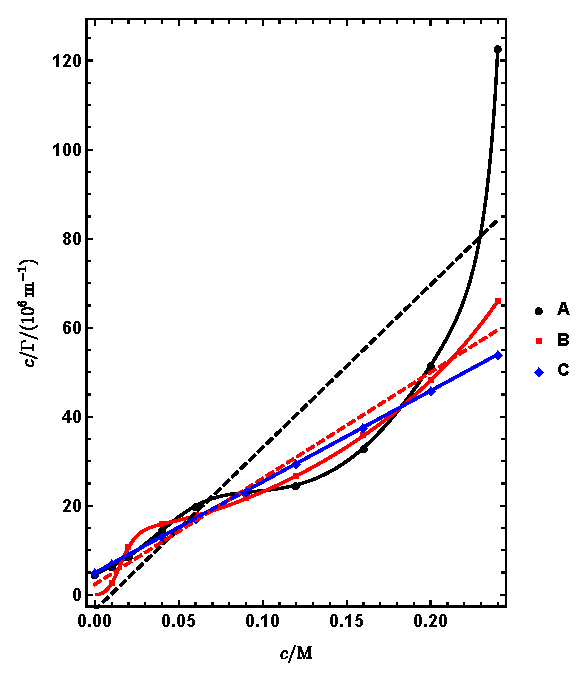
\includegraphics[width=0.45\textwidth]{figures/Langmuir.eps}
\caption{$\frac{c}{\Gamma}-c$ plots for three different fitting methods with their linear fits}
\label{Langmuir}
\end{figure}

The data is shown in Table.\ref{data}, with graphs of different statistical analyses given in Fig.\ref{fit}, \ref{Gibbs}, \ref{Langmuir}. 

The pressure is tranformed to $\gamma$ w.r.t. the surface tension of pure water, namely
\begin{equation}
\gamma_\text{water} = 75.75 - 0.145 T/\celsius + 0.000024 (T/\celsius)^2
\end{equation}
For fitting using power series of $c$, underfitting is evident in low degrees, with $R^2$ given by
\begin{equation*}
\begin{cases}
R_3^2 =0.993301 \\
R_4^2	= 0.997855 	\\
R_5^2		= 0.999006 	\\
R_6^2		= 0.999064
\end{cases}
\end{equation*}
where the lower indexes represent the degrees of power series used in the fitting, and 6 degrees might be the best fit for the data. For power series of $\ln{c}$, overfitting is conspicuous at high degrees, with $R^2$ given by
\begin{equation*}
\begin{cases}
R_2^2 =0.997561 \\
R_3^2	= 0.997887 \\
R_4^2		= 0.9994 \\
R_5^2		= 0.99945
\end{cases}
\end{equation*}
among which 3 degrees is the ideal one. The form of $C_1+C_2\ln{(c + C_3)}$ gives the best fitting result, with $R^2 = 0.999942$. The best fitting results from three different methods are given by
\begin{equation*}
\begin{cases}
72.23 - 527.5 c + 8106. c^2 - 81252. c^3 \\
\quad+ 439226. c^4 - 119256 c^5 + 128782 c^6\\
  50.45 + 29.27 \ln{c} + 24.72 \ln{^2c} + 6.317 \ln{^3c} + 0.5452 \ln{^4c} \\
  26.7642 - 12.1273 \ln{(c+ 0.0242117 )}
  \end{cases}
\end{equation*}
Gibbs isothermal lines in Fig.\ref{Gibbs} shows the similarity of the results between $A$ and $C$, with $B$ far away, which might be due to the numerical instability of $\ln{c}$ at $c\sim0$. Langmuir isothermal adsorption lines in Fig.\ref{Langmuir} gives the opposite result, indicating the similarity of the results between $B$ and $C$, with $B$ far away, which should be attributed to the numerical instability of $\frac{1}{c}$ at $c\sim0$. The linear fits of three methods are given by
\begin{equation*}
\begin{cases}
\left(\frac{c}{\Gamma}\right)_\text{A} = -3.43028 + 365.321 c ,\, R^2 = 0.755474\\
\left(\frac{c}{\Gamma}\right)_\text{B} = 2.34771 + 238.111 c ,\, R^2 =0.960557\\
\left(\frac{c}{\Gamma}\right)_\text{C} =  4.94886 + 204.4 c,\, R^2 =1.
\end{cases}
\end{equation*}
which reveals the reliability of the C method. Then
\begin{equation}
\begin{cases}
	\Gamma_\infty = 2.04 \times 10^{-5} \, \mathrm{mol \cdot m^{-2}}\\
	K = 0.0244 \,\mathrm{m} \\
	q = 0.0813 \,\mathrm{nm^2}
\end{cases}
\end{equation}
where $q$ is given by
\begin{equation}
q= \frac{1}{N_A \Gamma_\infty}
\end{equation}

Errors might be attributed to deviation from the state of perfect attachment of the capillary and the surface of the solution, as well as the delay of the measurement of pressure.

\section{Conclusion}
Surface tension of the different concentration of n-butanol solutions are obtained \emph{via} forming bubbles and measuring the deviation of pressure. Function form of $C_1+C_2\ln{(c + C_3)}$ fits the $\gamma-c$ plot best, giving superior linearity between $\frac{c}{\Gamma}$ and $c$, and thus the saturated adsorption amount as well as the cross-sectional area of n-butanol is obtained. 

\bibliography{References}
\end{document}
